\PassOptionsToPackage{unicode=true}{hyperref} % options for packages loaded elsewhere
\PassOptionsToPackage{hyphens}{url}
%
\documentclass[10pt,ignorenonframetext,]{beamer}
\usepackage{pgfpages}
\setbeamertemplate{caption}[numbered]
\setbeamertemplate{caption label separator}{: }
\setbeamercolor{caption name}{fg=normal text.fg}
\beamertemplatenavigationsymbolsempty
% Prevent slide breaks in the middle of a paragraph:
\widowpenalties 1 10000
\raggedbottom
\setbeamertemplate{part page}{
\centering
\begin{beamercolorbox}[sep=16pt,center]{part title}
  \usebeamerfont{part title}\insertpart\par
\end{beamercolorbox}
}
\setbeamertemplate{section page}{
\centering
\begin{beamercolorbox}[sep=12pt,center]{part title}
  \usebeamerfont{section title}\insertsection\par
\end{beamercolorbox}
}
\setbeamertemplate{subsection page}{
\centering
\begin{beamercolorbox}[sep=8pt,center]{part title}
  \usebeamerfont{subsection title}\insertsubsection\par
\end{beamercolorbox}
}
\AtBeginPart{
  \frame{\partpage}
}
\AtBeginSection{
  \ifbibliography
  \else
    \frame{\sectionpage}
  \fi
}
\AtBeginSubsection{
  \frame{\subsectionpage}
}
\usepackage{lmodern}
\usepackage{amssymb,amsmath}
\usepackage{ifxetex,ifluatex}
\usepackage{fixltx2e} % provides \textsubscript
\ifnum 0\ifxetex 1\fi\ifluatex 1\fi=0 % if pdftex
  \usepackage[T1]{fontenc}
  \usepackage[utf8]{inputenc}
  \usepackage{textcomp} % provides euro and other symbols
\else % if luatex or xelatex
  \usepackage{unicode-math}
  \defaultfontfeatures{Ligatures=TeX,Scale=MatchLowercase}
\fi
\usetheme[]{Luebeck}
\usecolortheme{whale}
\usefonttheme{structuresmallcapsserif}
% use upquote if available, for straight quotes in verbatim environments
\IfFileExists{upquote.sty}{\usepackage{upquote}}{}
% use microtype if available
\IfFileExists{microtype.sty}{%
\usepackage[]{microtype}
\UseMicrotypeSet[protrusion]{basicmath} % disable protrusion for tt fonts
}{}
\IfFileExists{parskip.sty}{%
\usepackage{parskip}
}{% else
\setlength{\parindent}{0pt}
\setlength{\parskip}{6pt plus 2pt minus 1pt}
}
\usepackage{hyperref}
\hypersetup{
            pdfauthor={Luisa Hammer and Marcelo Avila},
            pdfborder={0 0 0},
            breaklinks=true}
\urlstyle{same}  % don't use monospace font for urls
\newif\ifbibliography
\usepackage{longtable,booktabs}
\usepackage{caption}
% These lines are needed to make table captions work with longtable:
\makeatletter
\def\fnum@table{\tablename~\thetable}
\makeatother
\usepackage{graphicx,grffile}
\makeatletter
\def\maxwidth{\ifdim\Gin@nat@width>\linewidth\linewidth\else\Gin@nat@width\fi}
\def\maxheight{\ifdim\Gin@nat@height>\textheight\textheight\else\Gin@nat@height\fi}
\makeatother
% Scale images if necessary, so that they will not overflow the page
% margins by default, and it is still possible to overwrite the defaults
% using explicit options in \includegraphics[width, height, ...]{}
\setkeys{Gin}{width=\maxwidth,height=\maxheight,keepaspectratio}
\setlength{\emergencystretch}{3em}  % prevent overfull lines
\providecommand{\tightlist}{%
  \setlength{\itemsep}{0pt}\setlength{\parskip}{0pt}}
\setcounter{secnumdepth}{0}

% set default figure placement to htbp
\makeatletter
\def\fps@figure{htbp}
\makeatother

\widowpenalties 1 150
\newcommand{\begincols}[1]{\begin{columns}{#1}}
\newcommand{\stopcols}{\end{columns}}

\title{Replication of ``Educational Expansion and Its Heterogeneous Returns for
Wage Workers''\\
by\\
Michael Gebel and Friedhelm Pfeiffer}
\author{Luisa Hammer and Marcelo Avila}
\date{22 Nov 2018}

\begin{document}
\frame{\titlepage}

\hypertarget{theoretical-part}{%
\section{Theoretical Part}\label{theoretical-part}}

\begin{frame}{Summary of Gebel \& Pfeiffer (2010)}
\protect\hypertarget{summary-of-gebel-pfeiffer-2010}{}

\begin{itemize}
\tightlist
\item
  basic idea: examine evolution of returns to education in West German
  labour market.
\item
  Focus on change in returns to education over time as a consequence to
  education expansion in Germany.
\item
  methodology:

  \begin{itemize}
  \tightlist
  \item
    Wooldrigdge's (2004) \textbf{conditional mean independence}
  \item
    Garen's (1984) \textbf{control function} approach, that requires an
    \emph{exclusion restriction}
  \item
    as well as OLS
  \end{itemize}
\item
  data: SOEP 1984-2006
\end{itemize}

\end{frame}

\begin{frame}{Data and Variables}
\protect\hypertarget{data-and-variables}{}

\begin{itemize}
\tightlist
\item
  Log of hourly wage
\item
  Years of education (constructed from categorical variable)
\item
  Age and age squared
\item
  Gender
\item
  Father's education
\item
  Mother's education
\item
  Father's occupation
\item
  Rural or urban household
\item
  Number of Siblings (as instrument)
\end{itemize}

TODO: more detailed table? (Comment) not necessary (Comment) Leave data
intro when talking about the model later on?

\end{frame}

\begin{frame}{Background Information}
\protect\hypertarget{background-information}{}

\begin{itemize}
\item
  \textbf{increase in educational attainment} in the 1960s. From 1984 to
  2006, average years of schooling increased:

  \begin{itemize}
  \tightlist
  \item
    woman: 11.3 -\textgreater{} 12.8
  \item
    men: 11.9 -\textgreater{} 12.9
  \end{itemize}
\item
  \textbf{How can educational expansion affect the returns to
  education?}

  \begin{itemize}
  \tightlist
  \item
    Standard theory: an increase of labor supply of high-skilled workers
    should decrease the returns to education
  \item
    High-educated workers with higher unobserved motivation / ability
    which positively affects wages
  \item
    More ``less talented'' accepted to higher education \& thereby
    decreasing the average productivity levels of higher educated
    workers --\textgreater{} overall effect not clear
  \end{itemize}
\item
  unobserved characteristics leading to \textbf{selection bias}:

  \begin{itemize}
  \tightlist
  \item
    higher ability and motivation to stay longer in education
  \item
    select jobs with expected higher returns.
  \end{itemize}
\end{itemize}

\end{frame}

\hypertarget{econometric-approach}{%
\subsection{Econometric Approach}\label{econometric-approach}}

\begin{frame}[allowframebreaks]{Empirical Framework (Derivation)}
\protect\hypertarget{empirical-framework-derivation}{}

The study is based on the \textbf{correlated random coefficient model}
(Wooldridge, 2004) specified as: \[\ln Y_i = a_i + b_i S_i\] with
\(a_i = a'X_i + \varepsilon_{ai}\), and
\(b_i = b'X_i + \varepsilon_{bi}\)

where \(\ln Y_i\) : log of wages and \(S_i\) years of schooling of
individual \(i\)

\begin{itemize}
\item
  The model has, therefore, an \textbf{individual-specific intercept}
  \(a_i\) and \textbf{slope} \(b_i\) dependent on \textbf{observables}
  \(X_i\) and \textbf{unobservables} \(\varepsilon_{ai}\) and
  \(\varepsilon_{bi}\).
\item
  Do not assume that \(b_i\) and \(S_i\) are independent
  --\textgreater{} Individuals with higher expected benefits from
  education are more likely to remain longer in education
  --\textgreater{} \(b_i\) may be correlated with \(S_i\) indicating
  positive self-selection.
\item
  focus: estimate average partial effect (APE), which is the return per
  additional year of education for a randomly chosen individual (or
  averaged across the population)
  \[E(\partial \ln Y / \partial S) = E(b_i) = \beta\]
\end{itemize}

In case of homogeneous returns to education the wage equation reduces
to: \[\ln Y_i = a'X_i + \bar b S_i + \varepsilon_{ai}\] - Unobserved
heterogeneity may only affect the \textbf{intercept} of the wage
equation.

\begin{itemize}
\tightlist
\item
  still potential endogeneity if \(\varepsilon_{ai}\) correlates with
  \(S_i\)
\end{itemize}

\end{frame}

\begin{frame}{Empirical Framework (Intuition) I}
\protect\hypertarget{empirical-framework-intuition-i}{}

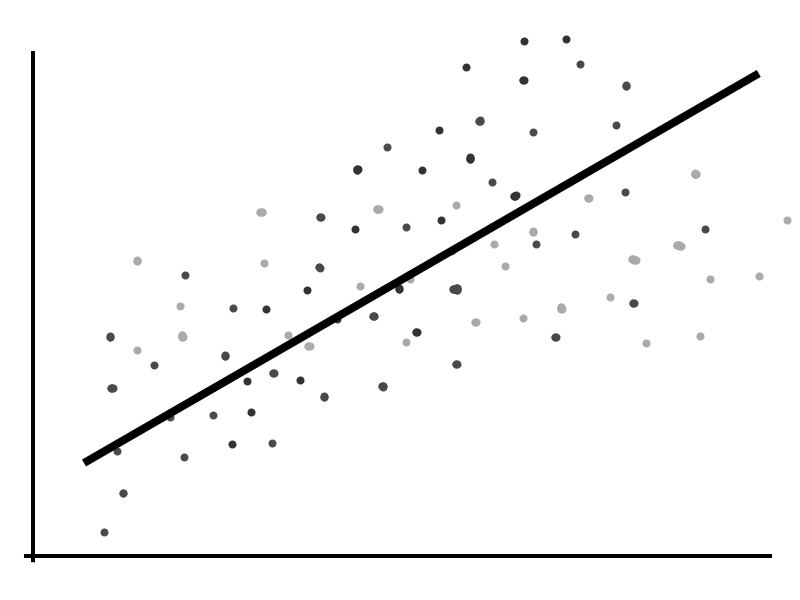
\includegraphics[width=3.125in,height=\textheight]{img/rcmodel001.png}

\begin{itemize}
\tightlist
\item
  Simple OLS
\end{itemize}

\end{frame}

\begin{frame}{Empirical Framework (Intuition) II}
\protect\hypertarget{empirical-framework-intuition-ii}{}

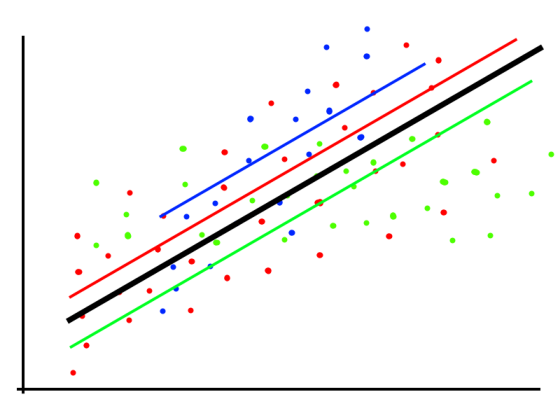
\includegraphics[width=3.125in,height=\textheight]{img/rcmodel002.png}

\begin{itemize}
\tightlist
\item
  Multiple OLS with homogeneous return to Educ
\end{itemize}

\end{frame}

\begin{frame}{Empirical Framework (Intuition) III}
\protect\hypertarget{empirical-framework-intuition-iii}{}

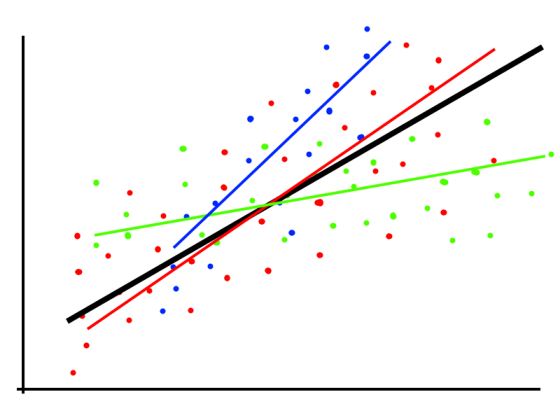
\includegraphics[width=3.125in,height=\textheight]{img/rcmodel003.png}

\begin{itemize}
\tightlist
\item
  Correlated Random Coefficient Model
\end{itemize}

\end{frame}

\begin{frame}{Distinction to conventional methods}
\protect\hypertarget{distinction-to-conventional-methods}{}

\begin{itemize}
\tightlist
\item
  OLS

  \begin{itemize}
  \tightlist
  \item
    ability and ``background'' bias
  \end{itemize}
\item
  IV Methods

  \begin{itemize}
  \tightlist
  \item
    if education is correlated with \textbf{unobserved individual
    heterogeneity}, IV methods may fail to identity APE.

    \begin{itemize}
    \tightlist
    \item
      alternative: \textbf{L}ocal \textbf{A}verage \textbf{T}reatment
      \textbf{E}ffect.
    \end{itemize}
  \end{itemize}
\end{itemize}

\end{frame}

\begin{frame}{Conditional Mean Independence}
\protect\hypertarget{conditional-mean-independence}{}

According to Wooldridge (2004, pg. 7), \textbf{APE} is identified by:
\[E (\ln Y_i \mid a_i, b_i, S_i, X_i,) = E (\ln Y_i \mid a_i, b_i, S_i) = a_i+b_i S_i \qquad (A.1)\]
\[E(S_i \mid a_i, b_i, X_i) = E(S_i \mid X_i) ~~\text{and}~~ \mathrm{Var}(S_i \mid 
a_i, b_i, X_i) = \mathrm{Var} (S_i \mid X_i) \qquad (A.2)\]

TODO: add interpretation of assumptions

\end{frame}

\begin{frame}{Estimator for \(\beta\) and GLM}
\protect\hypertarget{estimator-for-beta-and-glm}{}

\[\hat \beta = \frac{1}{N} \sum_{i=1}^N \left( \left( S_i - \hat E (S_i \mid X_i) \ln Y_i \right) \middle/
\hat{Var}(S_i \mid X_i)\right)\]

\[E(S_i \mid X_i ) = e^{\gamma X_i}  ~~~\text{and}~~~ Var(S_i \mid ) = \sigma^2e^{\gamma X_i}\]
Where \(\sigma^2\) can be consistently estimated by the mean of squared
Pearson residuals and standard errors are bootstrapped.

\end{frame}

\begin{frame}[allowframebreaks]{Control Function Approach}
\protect\hypertarget{control-function-approach}{}

\begin{itemize}
\tightlist
\item
  Based on proposition by Garen (1984).
\item
  Similar to Heckman two-step estimator.
\item
  Models schooling choice explicitly in first step
\item
  CF approach can identify APE in heterogeneous returns while standard
  IV approach may not.
\end{itemize}

First stage: modelling schooling choice

\[S_i = c'X_i + dZ_i + v_i ~~\text{with}~~ E(v_i \mid Z_i, X_i) = 0\]
where:

\begin{itemize}
\item
  \(X_i\) and \(Z_i\) influence the educational decision.
\item
  \(v_i\): Error term incorporating unobserved determinants of education
  choice.
\item
  \(Z_i\): Exclusion restriction (instrument).
\item
  \(V_i\), \(\varepsilon_{ai}\) and \(\varepsilon_{bi}\) are normally
  distributed with zero means and positive variances.
\item
  possible correlation between error terms
\item
  \(v_i\) is positive if an individual acquires higher education than
  expected conditional on observed characteristics
\end{itemize}

Second step: augmented wage equation
\[\ln Y_i = a_i + \beta S_i + \gamma_1 v_i + \gamma_2 V_iS_i + w_i
\] where:

\begin{itemize}
\item
  \(\gamma_1 v_i\) and \(\gamma_2\) are the \textbf{control functions}

  \begin{itemize}
  \item
    \(\gamma_1 = cov(\varepsilon_{ai}, v_i) /var(v_i)\)
  \item
    \(\gamma_2 = cov(\varepsilon_{bi}, v_i) /var(v_i)\)
  \end{itemize}
\item
  \(E(w_i \mid X_i, S_i, v_i) = 0\) (as shown in Heckman / Robb, 1985)
\end{itemize}

Interpretation of the coefficients of the control functions -
\(\gamma_1\) measures the effect of those unobserved factors that led to
over- or under-achievement in education on the wage - Thus, if
\(\gamma_1\) is positive, the unobserved factors affect schooling
\emph{and} wages positively - \(\gamma_2\) describes how this effect
changes with increasing levels of education - Positive coefficient would
indicate that those with unexpected educational ``over-achievement''
tend to earn higher wages

TODO: intuition for CF approach

\end{frame}

\hypertarget{replication-results}{%
\section{Replication results}\label{replication-results}}

\hypertarget{section}{%
\subsection{}\label{section}}

\begin{frame}{Set-up}
\protect\hypertarget{set-up}{}

\begin{itemize}
\tightlist
\item
  We use the same sample: West Germans (not foreign-born or
  self-employed) between 25 \& 60 years who work full-time
\item
  We have less observations than Gebel \& Pfeiffer (2010) per survey
  year after we delete all observations with missing values
\item
  Yet, we extend the observation period until 2016
\item
  Three estimation methods: OLS, CMI \& CF
\item
  We are not able to replicate the estimation results of Gebel \&
  Pfeiffer (2010) exactly, yet the trend / shape is similar
\end{itemize}

\end{frame}

\begin{frame}{Results}
\protect\hypertarget{results}{}

\begin{itemize}
\item
  I'm not so sure how to add images / tables here but in the new do-file
  link \url{https://1drv.ms/u/s!Ap1Tm8513oIthBjgylALS8Zp3A7G} you can
  just save the graph with all 3 approaches
\item
  \& then display on the other side the same graph from GP(2010, p.35)
\item
  also: here is a table with the our \& GP estimates for comparisons -
  your bootstrapped standard errors are already included
\end{itemize}

\url{https://1drv.ms/x/s!Ap1Tm8513oIthBp5BPId0qO8h3Yj}

\end{frame}

\begin{frame}{Estimated returns on education}
\protect\hypertarget{estimated-returns-on-education}{}

\begin{itemize}
\tightlist
\item
  Estimates from OLS \& CMI are similar, yet, CMI produces lower
  estimates which points to a positive self-selection bias
\item
  Generally, CF estimates are much more volatile and less precise
\end{itemize}

Differences between replicated \& original estimations - Our OLS
estimates are on average larger than those of Gebel \& Pfeiffer (2010)
by 0.004 percentage points - Our CMI estimates are on average larger
than those of Gebel \& Pfeiffer (2010) by 0.002 percentage points (first
years lower, than larger) - Our CF estimates are on average
significantly larger by 0.032 percentage points, though the divergence
gets smaller from 2000 onwards

\end{frame}

\begin{frame}[allowframebreaks]{Control function estimates}
\protect\hypertarget{control-function-estimates}{}

Instrumental variable in first stage - \emph{Number of siblings} is
significant at the 0.1\% level for all years - As expected, the number
of siblings has a negative impact on the years of schooling (the
estimates range between -0.13 \& -0.23) - We would assume that the
instrument does not directly affect the error term in the wage equation

Coefficients of the control functions - \(\gamma_1\) is negative for
majority of years, yet very small and insignificant in all years - Gebel
\& Pfeiffer (2010) estimate a positive coefficient in the 1980s and
1990s - but also insignificant - \(\gamma_2\) is negative and close to
zero for most years - Indicates that those with unexpectedly high
education have lower returns to education - Similarly, they are only
slightly significant in the 1980s, and stronger significant in the early
2000s - The estimates are very similar to those of Gebel \& Pfeiffer
(2010)

\begin{itemize}
\tightlist
\item
  that both coefficients are (mostly) negative hints that educational
  expansion caused more ``less able'' to achieve higher education
\end{itemize}

\end{frame}

\begin{frame}{Explanations for divergences between replication and Gebel
\& Pfeiffer (2010)}
\protect\hypertarget{explanations-for-divergences-between-replication-and-gebel-pfeiffer-2010}{}

\begin{itemize}
\tightlist
\item
  sample not the same
\item
  \ldots{}
\end{itemize}

\end{frame}

\begin{frame}{Pro's \& Con's of estimation methods}
\protect\hypertarget{pros-cons-of-estimation-methods}{}

\end{frame}

\begin{frame}{Results and Comparison I}
\protect\hypertarget{results-and-comparison-i}{}

\begin{figure}
\centering
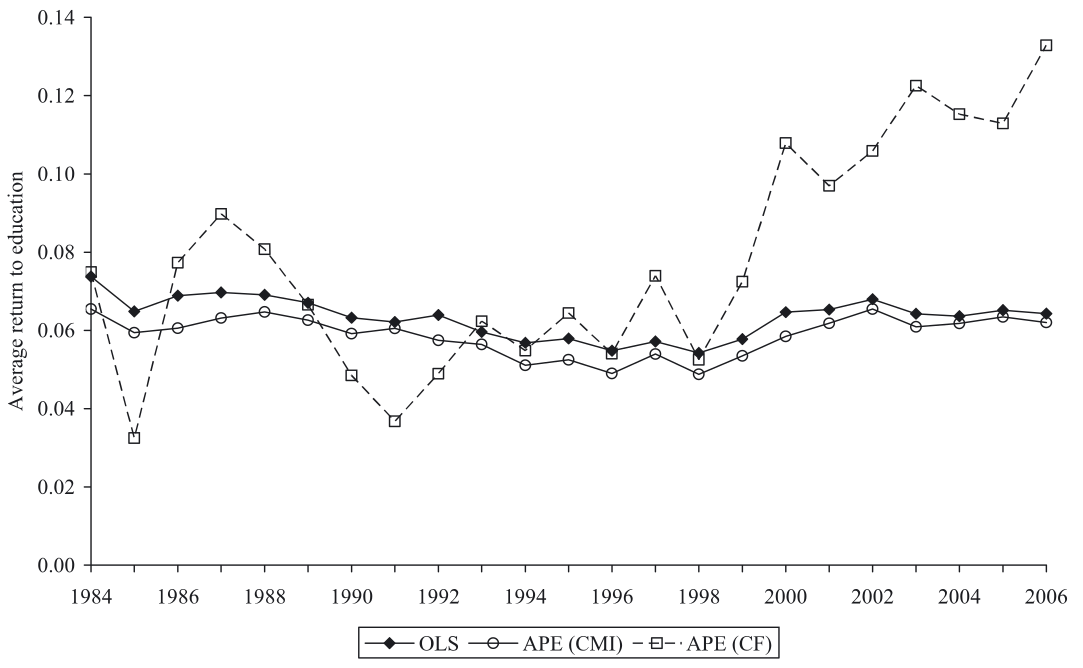
\includegraphics[width=\textwidth,height=2.60417in]{img/OLS_CMI_CF_GB2010.png}
\caption{Original Results (GB 2010, pg.30)}
\end{figure}

\end{frame}

\begin{frame}{Results and Comparison II}
\protect\hypertarget{results-and-comparison-ii}{}

\begin{figure}
\centering
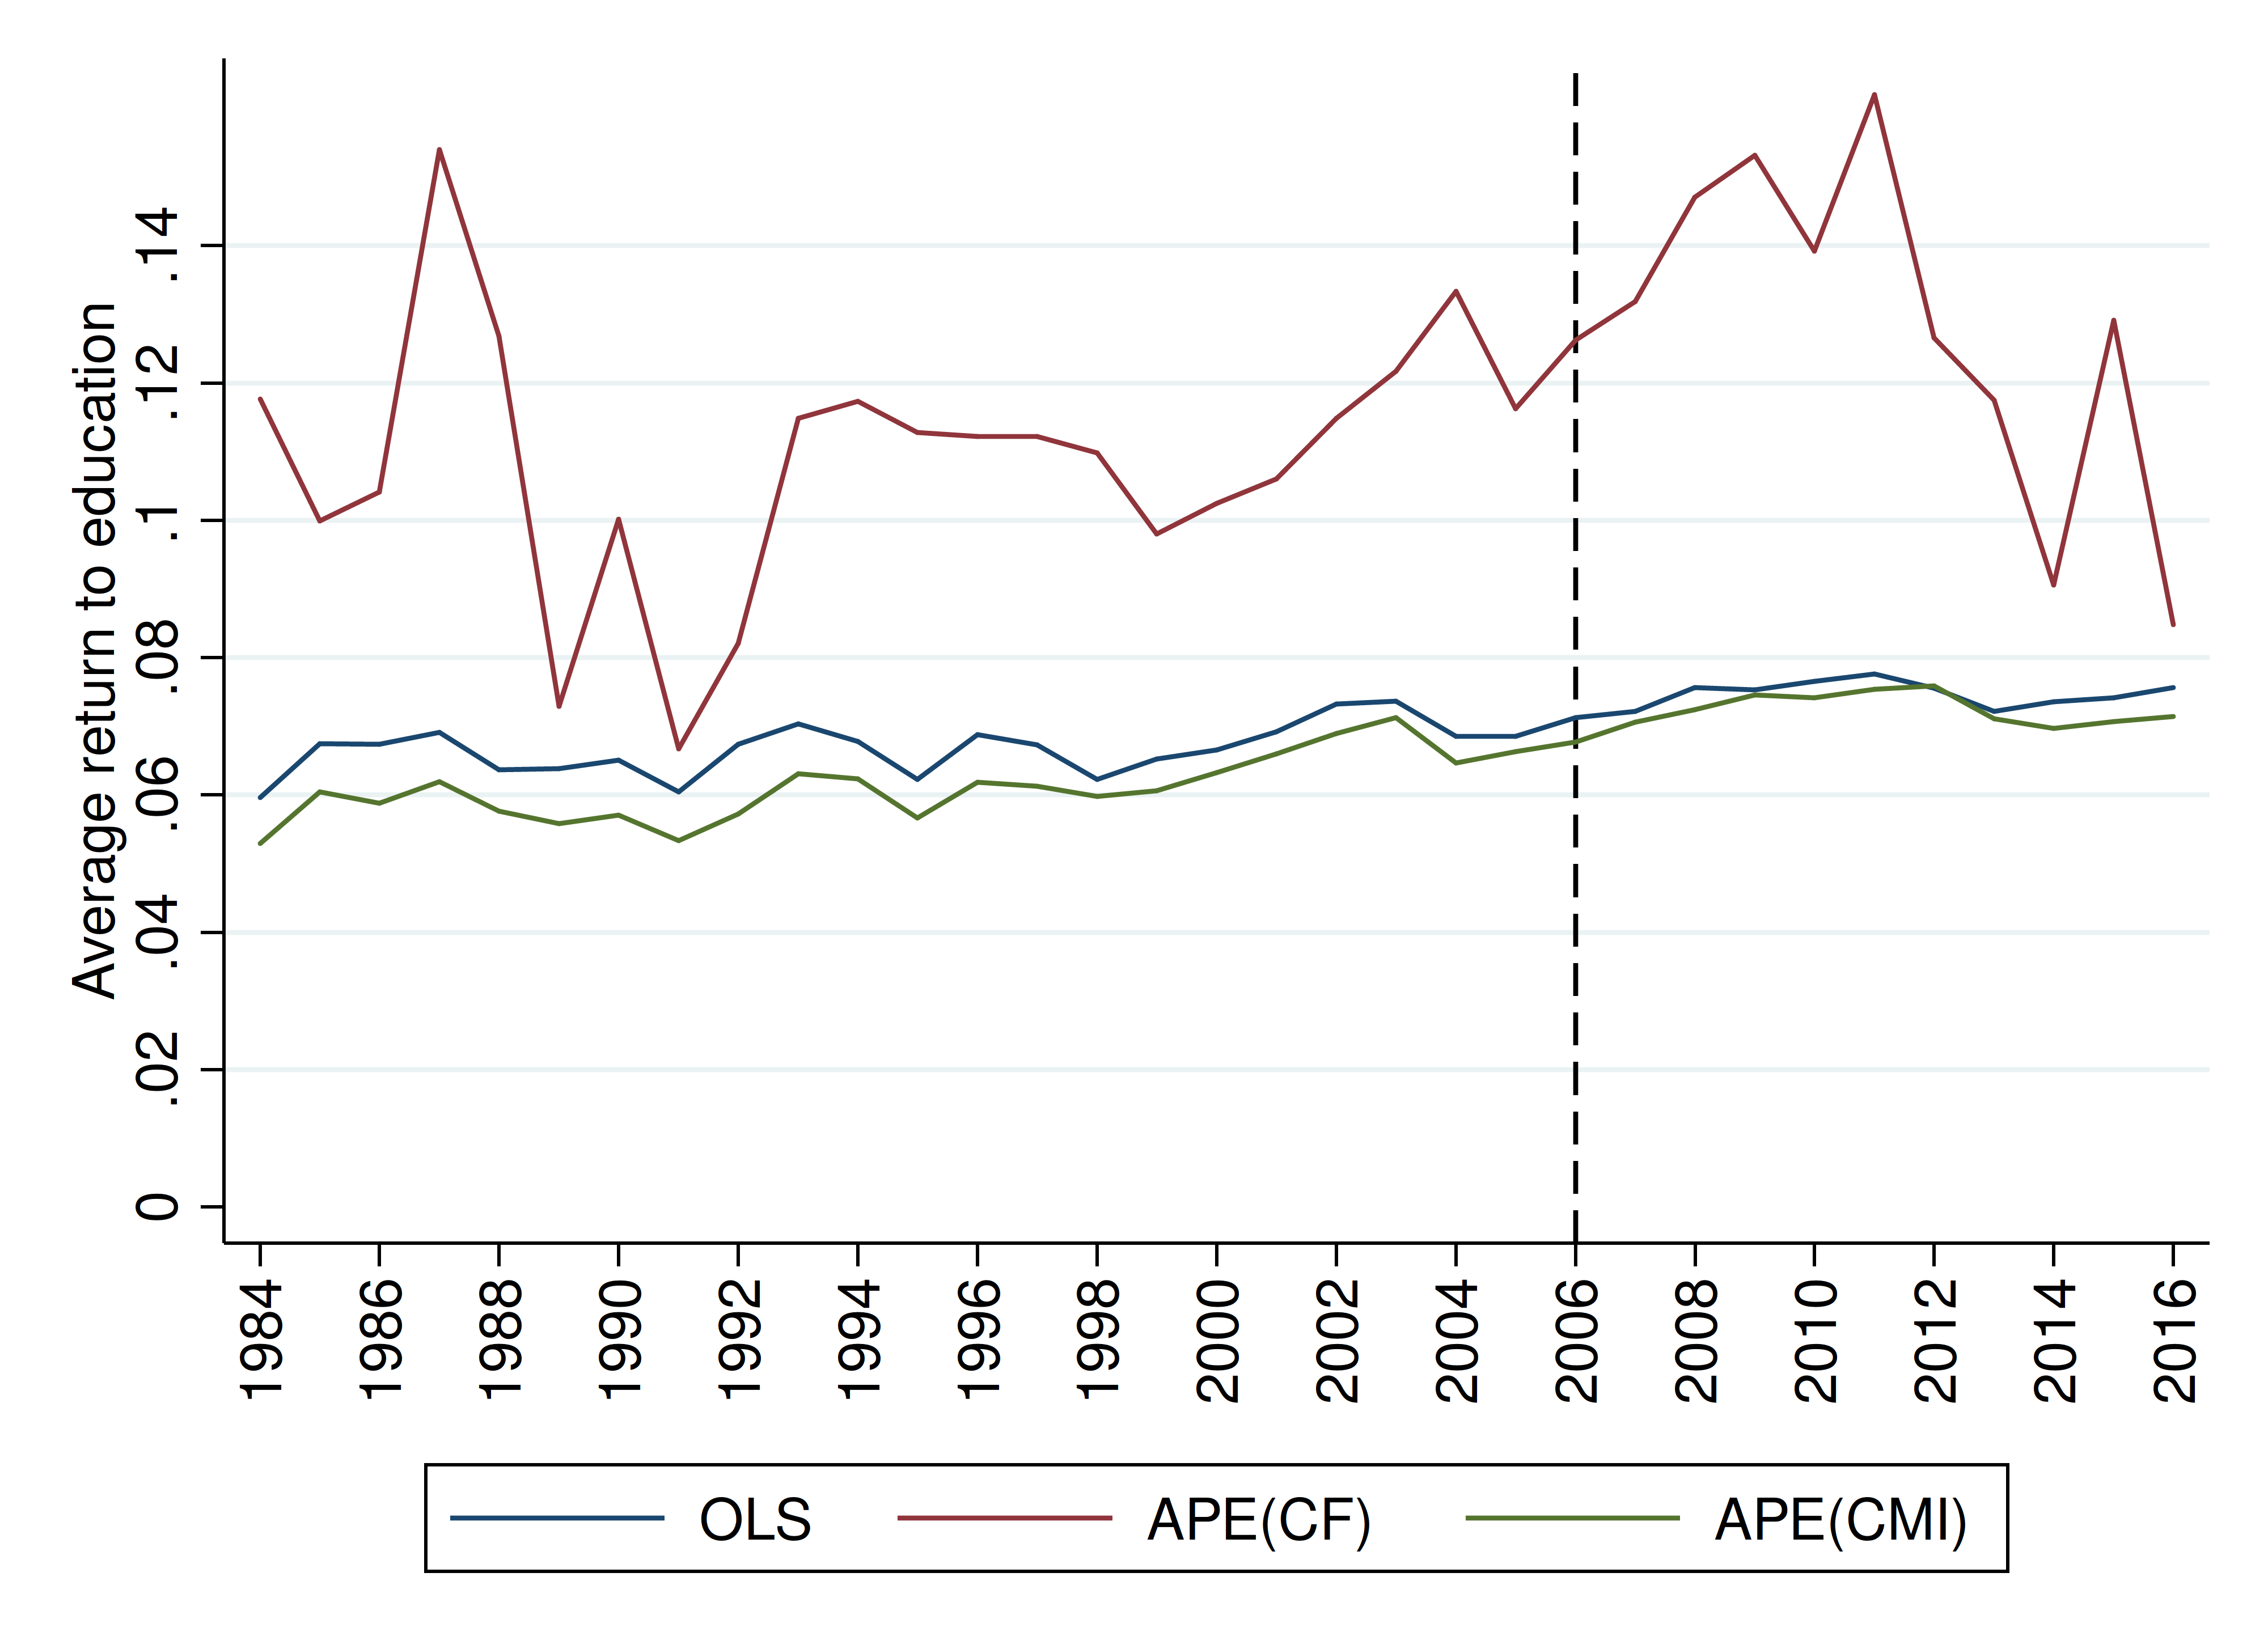
\includegraphics[width=\textwidth,height=2.60417in]{img/OLS_CMI_CF_Repli.png}
\caption{Replication results: Comparison between OLS, CMI and CF
approaches}
\end{figure}

\begingroup\fontsize{7}{9}\selectfont

\begin{longtable}{rrrrrrrrr}
\toprule
\multicolumn{1}{c}{ } & \multicolumn{2}{c}{First Stage} & \multicolumn{6}{c}{Second Stage} \\
\cmidrule(l{2pt}r{2pt}){2-3} \cmidrule(l{2pt}r{2pt}){4-9}
\multicolumn{1}{c}{ } & \multicolumn{2}{c}{IV: Nr. of Siblings} & \multicolumn{3}{c}{$v_i$} & \multicolumn{3}{c}{$v_i S_i$} \\
\cmidrule(l{2pt}r{2pt}){2-3} \cmidrule(l{2pt}r{2pt}){4-6} \cmidrule(l{2pt}r{2pt}){7-9}
year & coeff & s.e. & coeff.1 & s.e..1 & p & coeff.2 & s.e..2 & p.1\\
\midrule
\endfirsthead
\multicolumn{9}{@{}l}{\textit{(continued)}}\\
\toprule
\multicolumn{1}{c}{ } & \multicolumn{2}{c}{First Stage} & \multicolumn{6}{c}{Second Stage} \\
\cmidrule(l{2pt}r{2pt}){2-3} \cmidrule(l{2pt}r{2pt}){4-9}
\multicolumn{1}{c}{ } & \multicolumn{2}{c}{IV: Nr. of Siblings} & \multicolumn{3}{c}{$v_i$} & \multicolumn{3}{c}{$v_i S_i$} \\
\cmidrule(l{2pt}r{2pt}){2-3} \cmidrule(l{2pt}r{2pt}){4-6} \cmidrule(l{2pt}r{2pt}){7-9}
year & coeff & s.e. & coeff.1 & s.e..1 & p & coeff.2 & s.e..2 & p.1\\
\midrule
\endhead
\
\endfoot
\bottomrule
\endlastfoot
1984 & -0.163 & 0.035 & -0.019 & 0.036 & 0.601 & -0.003 & 0.001 & 0.027\\
1985 & -0.191 & 0.036 & 0.005 & 0.030 & 0.864 & -0.003 & 0.001 & 0.024\\
1986 & -0.129 & 0.034 & -0.039 & 0.041 & 0.344 & -0.001 & 0.001 & 0.681\\
1987 & -0.133 & 0.033 & -0.064 & 0.039 & 0.105 & -0.002 & 0.001 & 0.141\\
1988 & -0.150 & 0.034 & -0.031 & 0.034 & 0.365 & -0.003 & 0.001 & 0.038\\
\addlinespace
1989 & -0.153 & 0.033 & 0.018 & 0.033 & 0.590 & -0.002 & 0.001 & 0.056\\
1990 & -0.164 & 0.032 & -0.027 & 0.032 & 0.404 & -0.001 & 0.001 & 0.341\\
1991 & -0.167 & 0.033 & 0.014 & 0.034 & 0.685 & -0.002 & 0.001 & 0.152\\
1992 & -0.178 & 0.032 & -0.007 & 0.030 & 0.808 & -0.001 & 0.001 & 0.298\\
1993 & -0.162 & 0.033 & -0.033 & 0.033 & 0.311 & -0.001 & 0.001 & 0.264\\
\addlinespace
1994 & -0.176 & 0.034 & -0.035 & 0.029 & 0.233 & -0.001 & 0.001 & 0.225\\
1995 & -0.172 & 0.036 & -0.026 & 0.032 & 0.422 & -0.002 & 0.001 & 0.077\\
1996 & -0.195 & 0.037 & -0.015 & 0.031 & 0.624 & -0.003 & 0.001 & 0.058\\
1997 & -0.214 & 0.038 & -0.030 & 0.027 & 0.268 & -0.002 & 0.001 & 0.225\\
1998 & -0.200 & 0.036 & -0.049 & 0.028 & 0.076 & 0.000 & 0.001 & 0.866\\
\addlinespace
1999 & -0.219 & 0.036 & -0.029 & 0.027 & 0.282 & -0.001 & 0.001 & 0.559\\
2000 & -0.211 & 0.028 & -0.010 & 0.024 & 0.669 & -0.002 & 0.001 & 0.057\\
2001 & -0.191 & 0.027 & -0.007 & 0.023 & 0.769 & -0.002 & 0.001 & 0.021\\
2002 & -0.222 & 0.029 & 0.005 & 0.023 & 0.819 & -0.004 & 0.001 & 0.001\\
2003 & -0.209 & 0.029 & 0.016 & 0.024 & 0.499 & -0.005 & 0.001 & 0.000\\
\addlinespace
2004 & -0.228 & 0.029 & -0.025 & 0.024 & 0.298 & -0.003 & 0.001 & 0.006\\
2005 & -0.205 & 0.030 & -0.027 & 0.026 & 0.312 & -0.002 & 0.001 & 0.170\\
2006 & -0.213 & 0.030 & -0.032 & 0.026 & 0.221 & -0.002 & 0.001 & 0.107\\
2007 & -0.222 & 0.030 & -0.015 & 0.025 & 0.536 & -0.003 & 0.001 & 0.008\\
2008 & -0.226 & 0.031 & -0.048 & 0.027 & 0.082 & -0.002 & 0.001 & 0.149\\
\addlinespace
2009 & -0.206 & 0.031 & -0.026 & 0.028 & 0.343 & -0.004 & 0.001 & 0.004\\
2010 & -0.222 & 0.034 & -0.020 & 0.028 & 0.473 & -0.003 & 0.001 & 0.023\\
2011 & -0.215 & 0.032 & -0.029 & 0.028 & 0.297 & -0.004 & 0.001 & 0.001\\
2012 & -0.228 & 0.034 & 0.020 & 0.027 & 0.471 & -0.005 & 0.001 & 0.000\\
2013 & -0.224 & 0.033 & -0.005 & 0.028 & 0.857 & -0.003 & 0.001 & 0.017\\
\addlinespace
2014 & -0.238 & 0.035 & 0.015 & 0.028 & 0.579 & -0.003 & 0.001 & 0.038\\
2015 & -0.216 & 0.037 & -0.020 & 0.031 & 0.519 & -0.003 & 0.001 & 0.037\\
2016 & -0.212 & 0.038 & 0.027 & 0.034 & 0.423 & -0.003 & 0.001 & 0.037\\*
\end{longtable}\endgroup{}

\begingroup\fontsize{7}{9}\selectfont

\begin{longtable}{rrrrrrrl}
\toprule
year & OLS & OLS.se & CMI & CMI\_se & CF & CF\_se & obs\\
\midrule
\endfirsthead
\multicolumn{8}{@{}l}{\textit{(continued)}}\\
\toprule
year & OLS & OLS.se & CMI & CMI\_se & CF & CF\_se & obs\\
\midrule
\endhead
\
\endfoot
\bottomrule
\endlastfoot
1984 & 0.074 & 0.004 & 0.066 & 0.004 & 0.075 & 0.079 & 1.545\\
1985 & 0.065 & 0.004 & 0.059 & 0.004 & 0.032 & 0.131 & 1.600\\
1986 & 0.069 & 0.004 & 0.061 & 0.004 & 0.077 & 0.091 & 1.682\\
1987 & 0.070 & 0.004 & 0.063 & 0.004 & 0.090 & 0.048 & 1.775\\
1988 & 0.069 & 0.004 & 0.065 & 0.004 & 0.081 & 0.041 & 1.798\\
\addlinespace
1989 & 0.067 & 0.003 & 0.063 & 0.004 & 0.067 & 0.038 & 1.922\\
1990 & 0.063 & 0.003 & 0.059 & 0.004 & 0.048 & 0.031 & 2.007\\
1991 & 0.062 & 0.003 & 0.060 & 0.004 & 0.037 & 0.030 & 2.122\\
1992 & 0.064 & 0.003 & 0.057 & 0.004 & 0.049 & 0.027 & 2.107\\
1993 & 0.060 & 0.003 & 0.057 & 0.004 & 0.062 & 0.026 & 2.124\\
\addlinespace
1994 & 0.057 & 0.003 & 0.051 & 0.004 & 0.055 & 0.022 & 2.082\\
1995 & 0.058 & 0.003 & 0.053 & 0.004 & 0.064 & 0.024 & 2.075\\
1996 & 0.055 & 0.003 & 0.049 & 0.004 & 0.054 & 0.025 & 2.057\\
1997 & 0.057 & 0.003 & 0.054 & 0.003 & 0.074 & 0.025 & 2.011\\
1998 & 0.054 & 0.003 & 0.049 & 0.003 & 0.053 & 0.021 & 2.145\\
\addlinespace
1999 & 0.058 & 0.003 & 0.054 & 0.003 & 0.072 & 0.023 & 2.163\\
2000 & 0.065 & 0.002 & 0.059 & 0.003 & 0.108 & 0.024 & 3.965\\
2001 & 0.065 & 0.002 & 0.062 & 0.003 & 0.097 & 0.022 & 3.961\\
2002 & 0.068 & 0.003 & 0.066 & 0.003 & 0.106 & 0.030 & 3.668\\
2003 & 0.064 & 0.003 & 0.062 & 0.003 & 0.123 & 0.028 & 3.476\\
\addlinespace
2004 & 0.064 & 0.003 & 0.062 & 0.003 & 0.115 & 0.030 & 3.366\\
2005 & 0.065 & 0.003 & 0.064 & 0.003 & 0.113 & 0.032 & 3.220\\
2006 & 0.064 & 0.003 & 0.063 & 0.003 & 0.133 & 0.033 & 3.477\\*
\end{longtable}\endgroup{}

\begingroup\fontsize{7}{9}\selectfont

\begin{longtable}{rrrrrrrl}
\toprule
year & ret\_OLS & se\_OLS & se\_cf & ret\_cf & ret\_cmi & se\_cmi & obs\\
\midrule
\endfirsthead
\multicolumn{8}{@{}l}{\textit{(continued)}}\\
\toprule
year & ret\_OLS & se\_OLS & se\_cf & ret\_cf & ret\_cmi & se\_cmi & obs\\
\midrule
\endhead
\
\endfoot
\bottomrule
\endlastfoot
1984 & 0.060 & 0.004 & 0.030 & 0.118 & 0.053 & 0.006 & 1.448\\
1985 & 0.067 & 0.003 & 0.024 & 0.100 & 0.060 & 0.005 & 1.412\\
1986 & 0.067 & 0.004 & 0.036 & 0.104 & 0.059 & 0.006 & 1.463\\
1987 & 0.069 & 0.004 & 0.034 & 0.154 & 0.062 & 0.005 & 1.489\\
1988 & 0.064 & 0.003 & 0.029 & 0.127 & 0.058 & 0.005 & 1.476\\
\addlinespace
1989 & 0.064 & 0.003 & 0.028 & 0.073 & 0.056 & 0.005 & 1.553\\
1990 & 0.065 & 0.003 & 0.026 & 0.100 & 0.057 & 0.005 & 1.571\\
1991 & 0.060 & 0.004 & 0.028 & 0.067 & 0.053 & 0.005 & 1.602\\
1992 & 0.067 & 0.003 & 0.024 & 0.082 & 0.057 & 0.005 & 1.555\\
1993 & 0.070 & 0.004 & 0.027 & 0.115 & 0.063 & 0.005 & 1.527\\
\addlinespace
1994 & 0.068 & 0.003 & 0.024 & 0.117 & 0.062 & 0.005 & 1.491\\
1995 & 0.062 & 0.003 & 0.026 & 0.113 & 0.057 & 0.005 & 1.444\\
1996 & 0.069 & 0.003 & 0.025 & 0.112 & 0.062 & 0.005 & 1.383\\
1997 & 0.067 & 0.003 & 0.021 & 0.112 & 0.061 & 0.005 & 1.285\\
1998 & 0.062 & 0.003 & 0.022 & 0.110 & 0.060 & 0.005 & 1.452\\
\addlinespace
1999 & 0.065 & 0.003 & 0.021 & 0.098 & 0.061 & 0.005 & 1.452\\
2000 & 0.067 & 0.003 & 0.019 & 0.102 & 0.063 & 0.004 & 2.701\\
2001 & 0.069 & 0.003 & 0.019 & 0.106 & 0.066 & 0.004 & 2.659\\
2002 & 0.073 & 0.003 & 0.019 & 0.115 & 0.069 & 0.004 & 2.818\\
2003 & 0.074 & 0.003 & 0.020 & 0.122 & 0.071 & 0.004 & 2.741\\
\addlinespace
2004 & 0.069 & 0.003 & 0.018 & 0.133 & 0.065 & 0.004 & 2.558\\
2005 & 0.069 & 0.003 & 0.021 & 0.116 & 0.066 & 0.004 & 2.457\\
2006 & 0.071 & 0.003 & 0.020 & 0.126 & 0.068 & 0.004 & 2.525\\
2007 & 0.072 & 0.003 & 0.020 & 0.132 & 0.071 & 0.004 & 2.462\\
2008 & 0.076 & 0.003 & 0.021 & 0.147 & 0.072 & 0.005 & 2.316\\
\addlinespace
2009 & 0.075 & 0.003 & 0.023 & 0.153 & 0.075 & 0.004 & 2.367\\
2010 & 0.077 & 0.003 & 0.023 & 0.139 & 0.074 & 0.005 & 2.183\\
2011 & 0.078 & 0.003 & 0.023 & 0.162 & 0.075 & 0.004 & 2.523\\
2012 & 0.076 & 0.003 & 0.022 & 0.127 & 0.076 & 0.004 & 2.493\\
2013 & 0.072 & 0.003 & 0.022 & 0.117 & 0.071 & 0.004 & 2.477\\
\addlinespace
2014 & 0.074 & 0.003 & 0.022 & 0.091 & 0.070 & 0.004 & 2.353\\
2015 & 0.074 & 0.003 & 0.025 & 0.129 & 0.071 & 0.005 & 2.147\\
2016 & 0.076 & 0.003 & 0.028 & 0.085 & 0.071 & 0.005 & 1.971\\*
\end{longtable}\endgroup{}

\end{frame}

\begin{frame}[allowframebreaks]{The end}
\protect\hypertarget{the-end}{}

\end{frame}

\end{document}
